\documentclass[tikz,border=2pt]{standalone}
\usepackage{tikz}
\usepackage[scaled]{helvet}
\renewcommand{\familydefault}{\sfdefault}
\usepackage[T1]{fontenc}
\usepackage{mathptmx}
\usetikzlibrary{arrows.meta,bending}

\definecolor{leafred}{RGB}{220,75,75}
\definecolor{leafyellow}{RGB}{190,155,30}
\definecolor{leafcyan}{RGB}{40,180,190}
\definecolor{ctrcolor}{RGB}{220,140,40}

\tikzset{
  chord/.style={
    circle, draw=none, fill=#1, text=white,
    % WAS: circle, draw=white, line width=3pt, fill=#1, text=white,
    font=\bfseries\fontsize{22}{24}\selectfont\rmfamily, inner sep=2pt, minimum size=1.8cm},
  lbl/.style={font=\fontsize{12}{13.5}\selectfont\itshape,
              text width=3.0cm, align=center},
}

\begin{document}
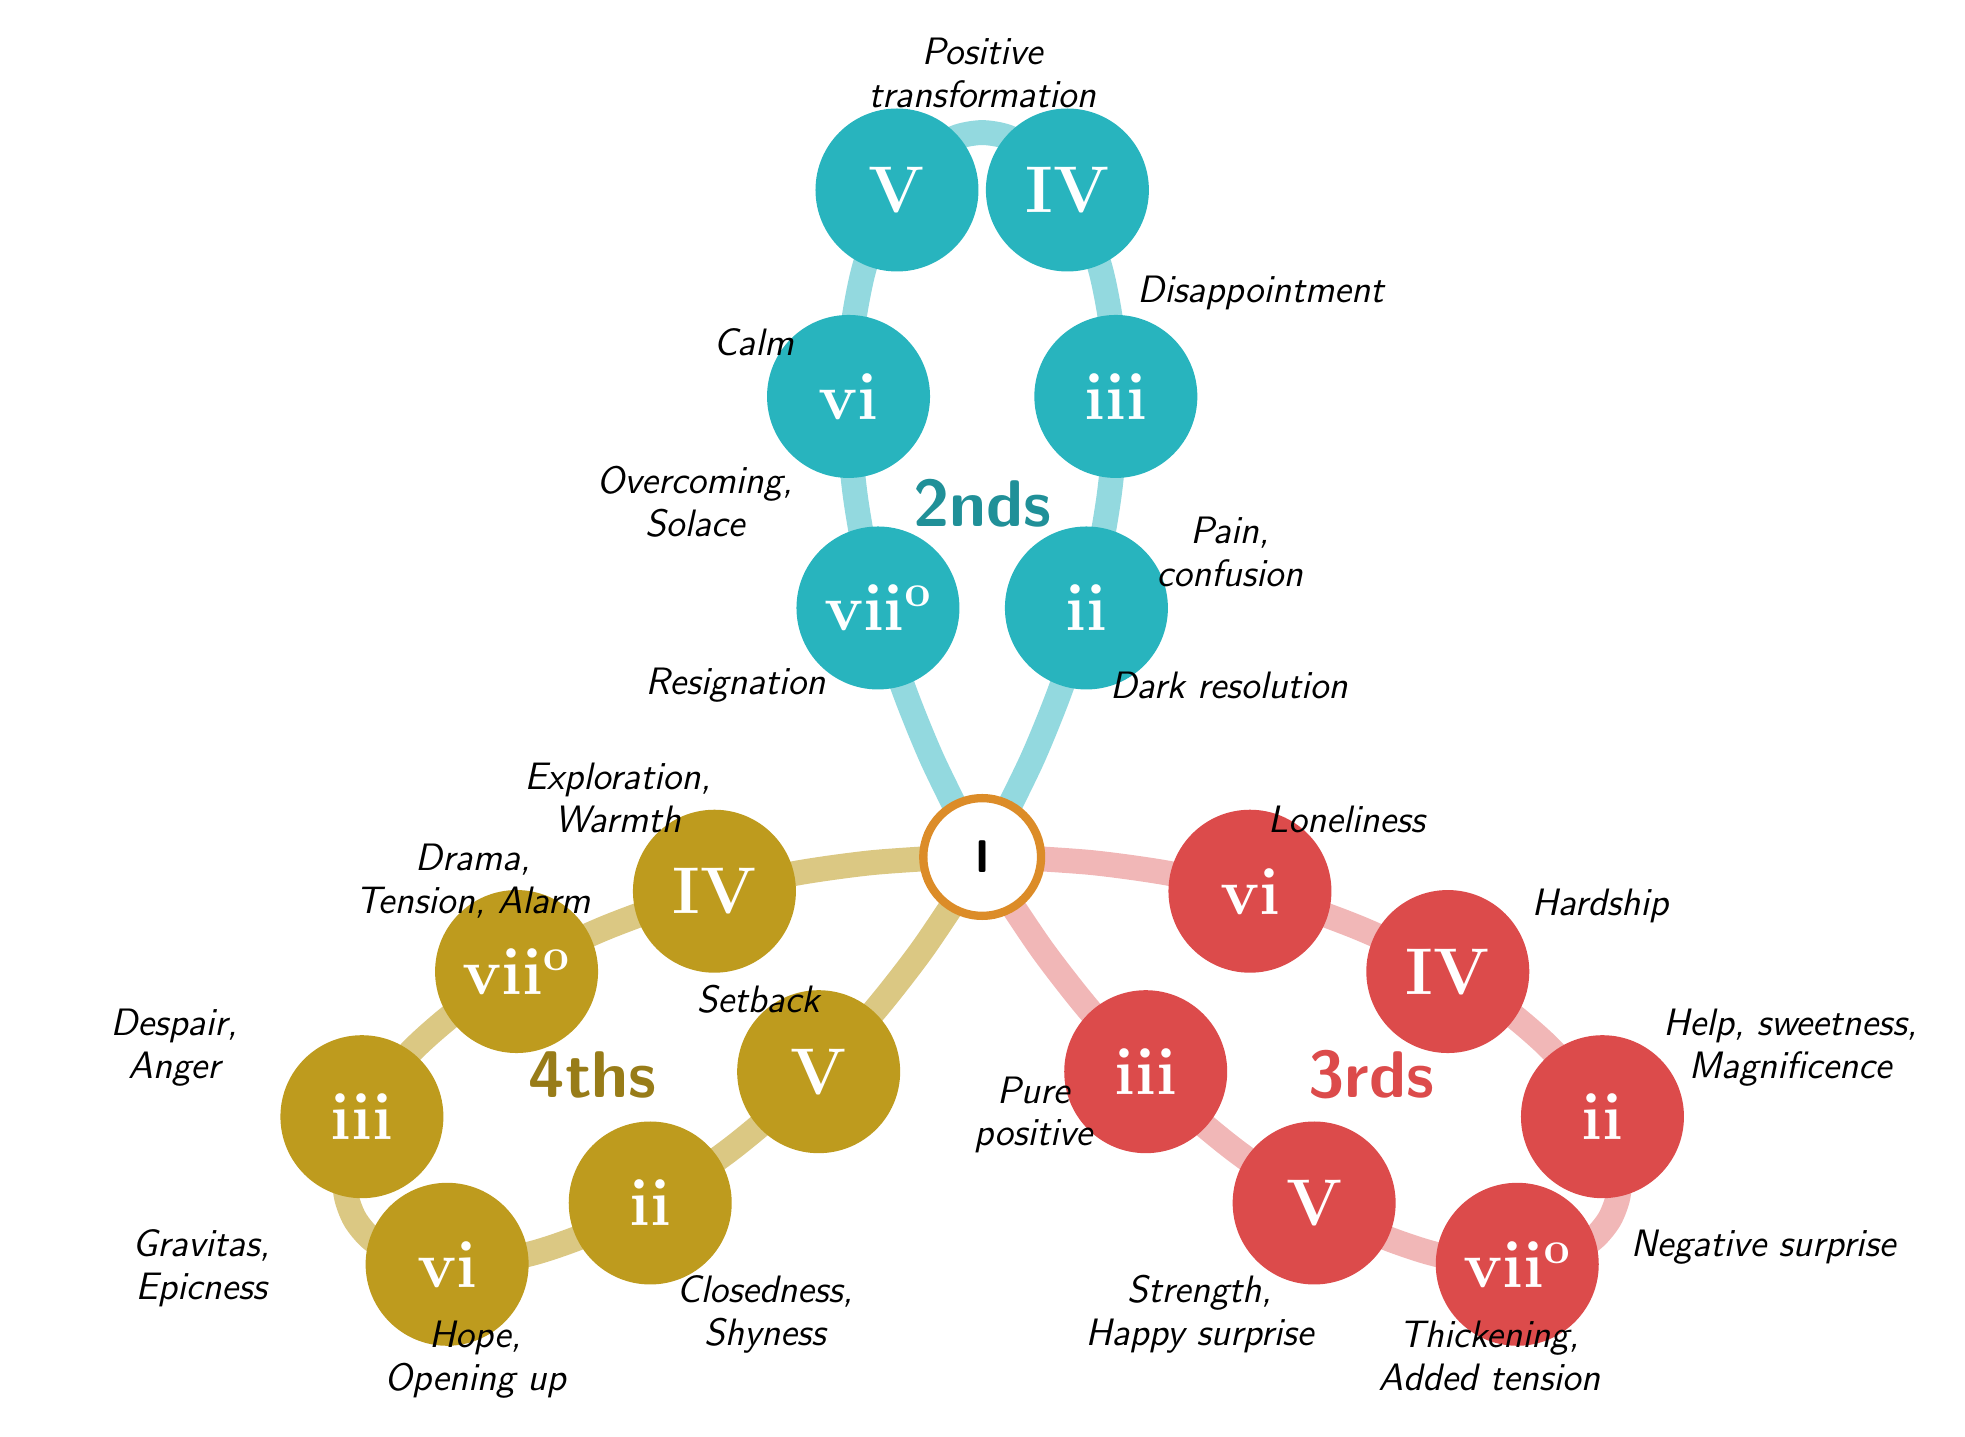
\begin{tikzpicture}[scale=1.15, every node/.style={transform shape}]

% Top leaf (2nds, cyan)
\draw[leafcyan!50, line width=9pt, line cap=round]
  plot[smooth, tension=0.5] coordinates {
  (0.203,0.366)(0.557,1.090)(0.856,1.826)(1.099,2.563)(1.281,3.292)
  (1.403,4.000)(1.466,4.679)(1.471,5.317)(1.421,5.906)(1.321,6.435)
  (1.175,6.898)(0.989,7.286)(0.771,7.595)(0.528,7.819)(0.269,7.955)
  (0.000,8.000)(-0.269,7.955)(-0.528,7.819)(-0.771,7.595)(-0.989,7.286)
  (-1.175,6.898)(-1.321,6.435)(-1.421,5.906)(-1.471,5.317)(-1.466,4.679)
  (-1.403,4.000)(-1.281,3.292)(-1.099,2.563)(-0.856,1.826)(-0.557,1.090)
  (-0.203,0.366)};

% Lower-left leaf (4ths, yellow)
\draw[leafyellow!55, line width=9pt, line cap=round]
  plot[smooth, tension=0.5] coordinates {
  (-0.419,-0.007)(-1.222,-0.063)(-2.009,-0.171)(-2.769,-0.330)(-3.491,-0.536)
  (-4.166,-0.785)(-4.785,-1.070)(-5.340,-1.384)(-5.825,-1.722)(-6.233,-2.074)
  (-6.561,-2.431)(-6.805,-2.786)(-6.963,-3.129)(-7.035,-3.452)(-7.023,-3.745)
  (-6.928,-4.000)(-6.755,-4.210)(-6.507,-4.367)(-6.192,-4.466)(-5.815,-4.500)
  (-5.386,-4.466)(-4.912,-4.361)(-4.404,-4.184)(-3.869,-3.933)(-3.319,-3.609)
  (-2.763,-3.216)(-2.210,-2.755)(-1.670,-2.233)(-1.153,-1.655)(-0.665,-1.027)
  (-0.216,-0.359)};

% Lower-right leaf (3rds, red)
\draw[leafred!40, line width=9pt, line cap=round]
  plot[smooth, tension=0.5] coordinates {
  (0.216,-0.359)(0.665,-1.027)(1.153,-1.655)(1.670,-2.233)(2.210,-2.755)
  (2.763,-3.216)(3.319,-3.609)(3.869,-3.933)(4.404,-4.184)(4.912,-4.361)
  (5.386,-4.466)(5.815,-4.500)(6.192,-4.466)(6.507,-4.367)(6.755,-4.210)
  (6.928,-4.000)(7.023,-3.745)(7.035,-3.452)(6.963,-3.129)(6.805,-2.786)
  (6.561,-2.431)(6.233,-2.074)(5.825,-1.722)(5.340,-1.384)(4.785,-1.070)
  (4.166,-0.785)(3.491,-0.536)(2.769,-0.330)(2.009,-0.171)(1.222,-0.063)
  (0.419,-0.007)};

%% Center
\node[circle, draw=ctrcolor, line width=3pt, fill=white,
      font=\bfseries\Large, minimum size=1.3cm] (C) at (0,0) {I};

%% == 2NDS (top) ==============================================================
\node[chord=leafcyan]         at ( 1.151, 2.750) {ii};
\node[chord=leafcyan]         at ( 1.476, 5.086) {iii};
\node[chord=leafcyan]         at ( 0.941, 7.366) {IV};
\node[chord=leafcyan]         at (-0.941, 7.366) {V};
\node[chord=leafcyan]         at (-1.476, 5.086) {vi};
\node[chord=leafcyan]         at (-1.151, 2.750) {vii\textsuperscript{o}};
\node[font=\bfseries\huge, leafcyan!80!black] at (0, 3.9) {2nds};

% I->ii: right side, between I and ii
\node[lbl, anchor=west]  at ( 1.1, 1.9) {Dark resolution};
% ii->iii
\node[lbl, anchor=west]  at ( 1.11, 3.37) {Pain,\\ confusion};
% iii->IV
\node[lbl, anchor=west]  at ( 1.45, 6.23) {Disappointment};
% IV->V (tip)
\node[lbl, anchor=south] at ( 0.00, 8.15) {Positive\\ transformation};
% V->vi
\node[lbl, anchor=east]  at (-0.9, 5.68) {Calm};
% vi->viio
\node[lbl, anchor=east]  at (-1.55, 3.92) {Overcoming,\\ Solace};
% viio->I: left side, between viio and I
\node[lbl, anchor=east]  at (-1.1, 1.9) {Resignation};

%% == 4THS (lower-left) =======================================================
\node[chord=leafyellow]       at (-2.957,-0.378) {IV};
\node[chord=leafyellow]       at (-5.142,-1.265) {vii\textsuperscript{o}};
\node[chord=leafyellow]       at (-6.850,-2.868) {iii};
\node[chord=leafyellow]       at (-5.909,-4.498) {vi};
\node[chord=leafyellow]       at (-3.666,-3.821) {ii};
\node[chord=leafyellow]       at (-1.806,-2.371) {V};
\node[font=\bfseries\huge, leafyellow!80!black] at (-4.3,-2.4) {4ths};

% I->IV: in gap between 2nds and 4ths leaves
\node[lbl, anchor=south east] at (-2.4, 0.15)    {Exploration,\\ Warmth};
% IV->viio
\node[lbl, anchor=south east] at (-4.0,-0.8)    {Drama,\\ Tension, Alarm};
% viio->iii
\node[lbl, anchor=east]       at (-7.3,-2.1)    {Despair,\\ Anger};
% iii->vi (tip)
\node[lbl, anchor=north east] at (-7.0,-4.0)    {Gravitas,\\ Epicness};
% vi->ii
\node[lbl, anchor=north]      at (-5.6,-5.0)    {Hope,\\ Opening up};
% ii->V
\node[lbl, anchor=north]      at (-2.4,-4.5)    {Closedness,\\ Shyness};
% V->I: in gap between 4ths and 3rds leaves
\node[lbl, anchor=north east] at (-0.85,-1.3)    {Setback};

%% == 3RDS (lower-right) ======================================================
\node[chord=leafred]          at ( 1.806,-2.371) {iii};
\node[chord=leafred]          at ( 3.666,-3.821) {V};
\node[chord=leafred]          at ( 5.909,-4.498) {vii\textsuperscript{o}};
\node[chord=leafred]          at ( 6.850,-2.868) {ii};
\node[chord=leafred]          at ( 5.142,-1.265) {IV};
\node[chord=leafred]          at ( 2.957,-0.378) {vi};
\node[font=\bfseries\huge, leafred] at ( 4.3,-2.4) {3rds};

% I->iii: in gap between 4ths and 3rds leaves
\node[lbl, anchor=north west] at (-1.06,-2.3)    {Pure\\ positive};
% iii->V
\node[lbl, anchor=north]      at ( 2.4,-4.5)    {Strength,\\ Happy surprise};
% V->viio
\node[lbl, anchor=north]      at ( 5.6,-5.0)    {Thickening,\\ Added tension};
% viio->ii (tip)
\node[lbl, anchor=north west] at ( 7.0,-4.0)    {Negative surprise};
% ii->IV
\node[lbl, anchor=west]       at ( 7.3,-2.1)    {Help, sweetness,\\ Magnificence};
% IV->vi: in gap between 3rds and 2nds leaves
\node[lbl, anchor=south west] at ( 5.2,-0.85)    {Hardship};
% vi->I: in gap between 3rds and 2nds leaves
\node[lbl, anchor=south west] at ( 2.4, 0.15)    {Loneliness};

%% == HYMNAL STATS (v5g, 288 hymns, 3,014 transitions) =========================
%% Positioned below the trefoil
\end{tikzpicture}

\end{document}
